\documentclass[entwurf.tex]{subfiles}

\begin{document}
\chapter{Klassendiagramme}
	\section{Bus}
		\begin{figure}[H]
  			\begin{center}
 				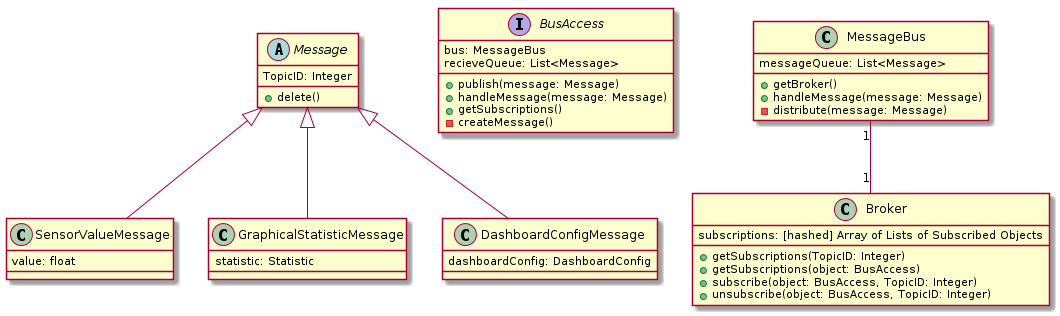
\includegraphics[width=0.8\textheight,angle=90]{diagrams/Bus.png}
  				\caption{Bus Klassendiagramm}
  			\end{center}
  		\end{figure}
  		In diesem Diagramm ist der Aufbau des Moduls ''Bus'' zu sehen. Die Kommunikation aller Module ist entkoppelt und findet größtenteils über den Austausch von Nachrichten verschiedener Typen über den Bus statt. Um mit dem Bus arbeiten zu können, muss ein Modul eine Klasse besitzen, die von ''BusAccess'' erbt. Der Bus funktioniert als eine Variation des Beobachter-Entwurfsmusters. Eine von ''BusAccess'' erbende Klasse kann über subscribe() bzw. unsubscribe() auf dem ''MessageBus'' Nachrichten eines bestimmten Topics (Sensortyp, Datenbanknachrichten, Konfigurationsnachrichten) abonnieren. \\
  		Diese Abbonements werden in der Klasse ''Broker'' verwaltet. Sendet ein Objekt von ''BusAccess'' über publish() eine Nachricht an ''MessageBus'', so holt sich letzterer von seinem Broker eine Liste über alle Abonnements für das Topic der Nachricht und sendet diese dann an alle abonnierenden Objekte. Das versenden einer Nachricht sowie deren Empfang sind asynchrone Funktionsaufrufe. \\
  		Die Oberklasse ''Message'' besitzt eine Reihe von erbenden Klassen. Dies ist nötig, um alle möglichen Typen von Nachrichten darzustellen: ''SensorValueMessage'' wird für das einfache versenden von Messwerten benutzt, ''ConfigFileRequest'' für Konfigurationsdateien usw. Dieser Aufbau ermöglicht das leichte Ergänzen um ggf. zusätzlich benötigte Nachrichtentypen. Ein besonderer Nachrichtentyp ist die DatabaseRequestMessage, die Anfragen an die Datenbank beinhaltet. Die Anfragen vom Typ ''DBRequest'' sind unterteilt in verschiedene Typen von Anfragen: DBReqRecent fordert die letzten n Einträge an, DBReqFrom alle Einträge seit einem Datum, und DBReqRange fordert alle Datenbankeinträge zwischen zwei Daten an. \\
  		Das Konstrukt  der Klassen ''BusAccess'' sowie erbende Klassen, ''Message'' und die von ''Message'' erbenden Klassen ergeben gemeinsam das Entwurfsmuster der Fabrikmethode. 
  		
  	
  	\newpage
  	\section{Virtual Sensors}
		Hier sieht man den Aufbau der Virtuellen Sensoren.
		\begin{figure}[H]
  			\begin{center}
 				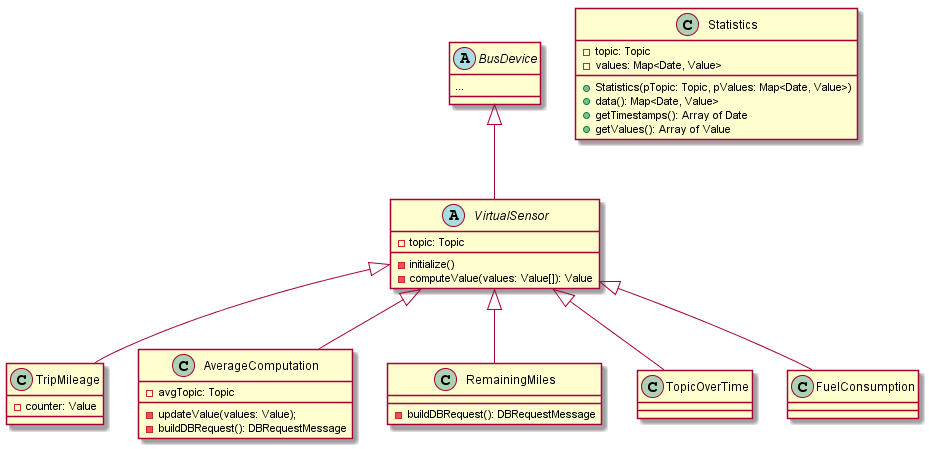
\includegraphics[width=0.8\textheight,angle=90]{diagrams/VirtualSensors.png}
  				\caption{Virtuelle Sensoren Klassendiagramm}
  			\end{center}
  		\end{figure}
  		
  	\section{Database Access}
  		Im folgenden Diagramm ist der Aufbau der Datenbank und des Datenbankzugriffs zu sehen.
  		\begin{figure}[H]
  			\begin{center}
 				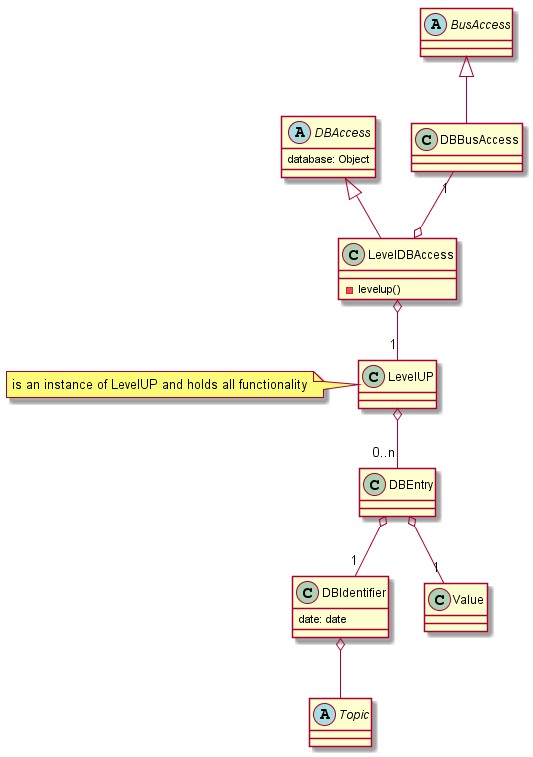
\includegraphics[height=0.8\textheight]{diagrams/DBAccess.png}
  				\caption{Virtuelle Sensoren Klassendiagramm}
  			\end{center}
  		\end{figure}
  	Als Datenbank wurde, wie im Pflichtenheft spezifiziert, LevelDB benutzt. Die Access-Klasse für LevelDB erbt von einer ''DBAccess''-Oberklasse, um leichte Austauschbarkeit zu gewährleisten. In der LevelDBAccess-Klasse wird außer der Referenz auf die LevelUp-Instanz auch der aktuelle Fahrer sowie die spezifizierte maximale Kapazität der Datenbank gehalten. \\ In der Datenbank, im Fall von LevelDB ein einfacher Key-Value-Store, werden zwei Typen von Objekten gehalten: Zum einen werden mit der Zeit und dem Typ des Sensors als Key Objekte von Sensorwerten und Fahrer gespeichert, zum anderen fahrerbezogene Einträge, die präferierten Kraftstoff und eine Referenz auf die Konfiguration des virtuellen Armaturenbretts mit der Identifikation des Fahrers als Key gespeichert werden. Zur Kommunikation mit anderen Modulen besitzt der Datenbankzugriff mit DBBusAccess eine Klasse, die den Zugang zum Bus möglich macht und Nachrichten vom Bus dekodiert. 
  	

	\newpage
  	\section{Website}
  	\label{Class:Website}
		Hier ist zu sehen wie die Seite allgemein aufgebaut ist. Die Website besteht aus zwei Frames. In einem wird die Statusbar angezeigt, im anderen werden können verschiedene Views sichtbar sein. Unter anderem z.B. das GridView auf dem die Dashes angezeigt werden. Für weiteres siehe: TODO %TODO Add UserInterface, ParkingView, MapView
Die Statusbar kann aus mehreren Buttons, Text und Icons bestehen.
		\begin{figure}[H]
  			\begin{center}
 				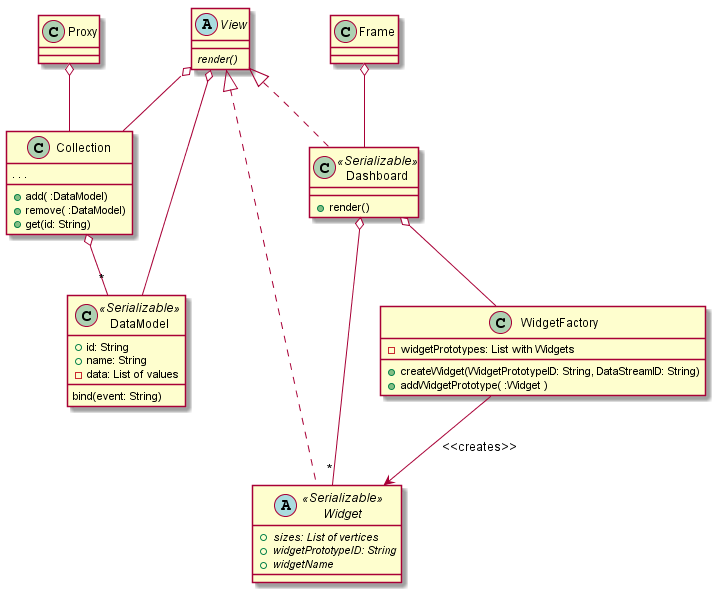
\includegraphics[width=\textwidth]{diagrams/website.png}
  				\caption{UI Klassendiagramm}
  			\end{center}
  		\end{figure}  	
  	
  	\newpage
  	\section{User Interface}
		Wie in \ref{Class:Website} zu sehen ist besteht ein Hauptteil des UserInterface aus dem ViewFrame der von verschiedenen Views vertreten werden kann. Hier sieht man den Aufbau des GridViews und des SettingViews. Das Grid nutzt eine Objekt der Klasse Gridster die aus der Bibliothek Gridster stammt. Das GridView besteht hauptsächlich aus diesem Objekt. Es ermöglicht verschiedene Widgets in einem Grid mit Elementen verschiedener Größen dynamisch anzeigen zu lassen.
		
		Hierbei sind die Widgets selbst Abonnenten des angezeigten Signals, weshalb diese die Abstrakte Klasse BusAccess implementieren müssen.
		
		Über die SettingsView ist es möglich verschiedene Widgets in dieses Grid hinzuzufügen oder zu ändern. Weshalb sich das SettingView immer die Instanz des Grids als Objekt speichert. Dies kommt zum Einsatz wenn z.B. ein früherer Zustand des Serializable Grids wiederhergestellt werden soll. Um früher gespeicherte Konfigurationen vom Bus zu empfangen und neue Einstellungen an den Server zu schicken implementiert auch die SettingsView den BusAccess. 
		
		
		\begin{figure}[H]
  			\begin{center}
 				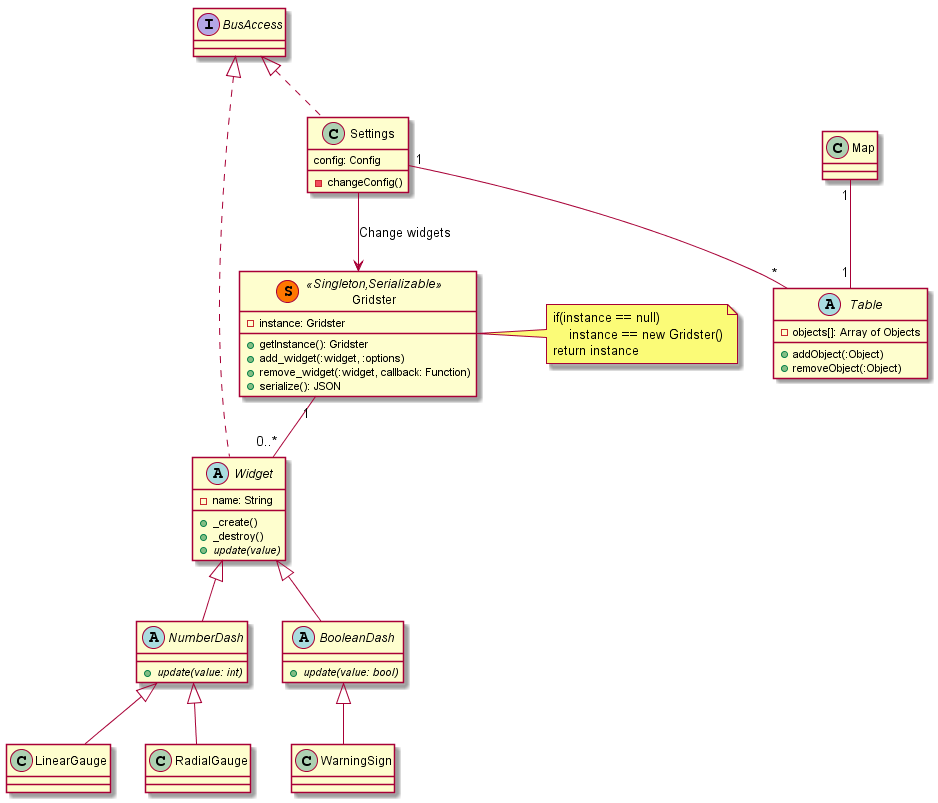
\includegraphics[width=\textwidth]{diagrams/UI.png}
  				\caption{UI Klassendiagramm}
  			\end{center}
  		\end{figure}
  		
  		
  		
  	\newpage
  	\section{Parking Sensor}
		Hier ist zu sehen wie das Rückfahrassistenzsystem aufgebaut ist. Siehe auch %TODO Link sequenzdiagramm
		\begin{figure}[H]
 			%\makebox[\textwidth][c]{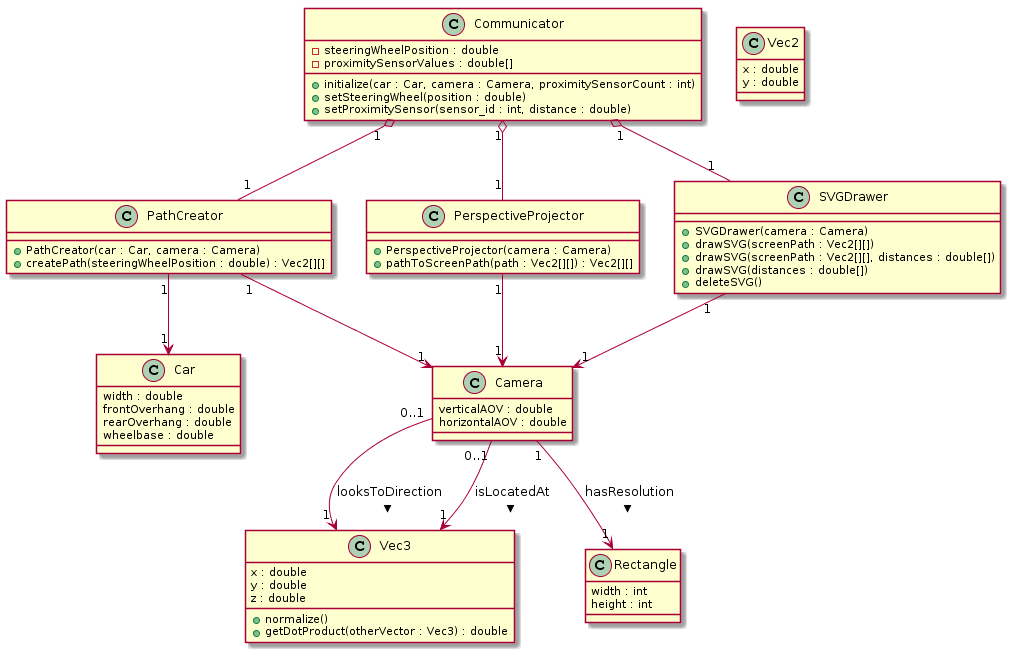
\includegraphics[width=0.9\paperwidth]{diagrams/ParkingSensor/class_diagram.png}}
  			\caption{Rückfahrsystem Klassendiagramm}
  		\end{figure}
  	
  	
\chapter{Klassen}
	\section{BusAccess}
	\label{Class:BusAccess}
		Eine abstrakte Klasse die es ermöglichen soll Zugriff auf den Bus zu bekommen.
		\begin{description}
			\attr{private messages: List of Messages} 
				Noch zu versendende Nachrichten
			\method{public publish(message: Message): Boolean} 
				Veröffentliche eine Nachricht.\\ 
				\textbf{Rückgabewert:} Erfolg des Veröffentlichen?
			\method{abstract public handleMessage(message: Message)} 
				Funktion zum empfangen einer neuen und abonnierten Nachricht.\\ 
				\textbf{Rückgabewert:}
			\method{public subscribe(object: BusAccess, topic: Topic): boolean} 
				Funktion um ein Topic zu abonnieren.\\ 
				\textbf{Parameter:} Der Abonnent und das abonnierte Topic.\\ 
				\textbf{Rückgabewert:} Erfolg des abonnierens.
			\method{public unsubscribe(object: BusAccess, topic: Topic): boolean} 
				Funktion um ein Abonnement zu beenden.\\ 
				\textbf{Parameter:} Der Abonnent und das abonnierte Topic.\\ 
				\textbf{Rückgabewert:} Erfolg des beendens
			\method{private createMessage(): Message}
				Ganz ehrlich: Ich hab keine Ahnung für was die hier sein soll. Da sollte vllt noch ein oder zwei Parameter zum erzeugen der Message.
		\end{description}
  		
	\section{Message}
	\label{Class:Message}
		Eine abstrakte Klasse die als Muster für alle Nachrichten auf dem Bus genutzt wird.
		\begin{description}
			\attr{protected topic: Topic} 
				Das Topic der Nachricht.
		\end{description}
		

  	
\end{document}
